\documentclass{article}

\usepackage{fullpage}
\usepackage{amssymb}
\usepackage{amsmath}
\usepackage{amsfonts}
\usepackage{mathrsfs}
\usepackage{graphicx}
\usepackage{minted}
\usepackage{multicol}
\usepackage{tikz}
\usepackage{hyperref}

\author{Anthony LaTorre}
\date{\today}

\title{SNO+ Scintillation}

\newcommand{\like}{\mathscr{L}}
\newcommand{\N}{\mathrm{N}}

\begin{document}
\maketitle

\begin{abstract}
    In this paper I find an analytic expression for the time distribution at
    the edge of a spherical detector for light emitted with an exponential time
    distribution within the detector. I show how this distribution can be used
    to fit for the radius of an event from only the hit times of all PMTs, and
    find that it is possible to reconstruct the radius with a resolution of
    approximately 2cm at a radius of 1m from 1200 photons. I also show how the
    distribution can be used as a cut to filter out non-scintillation events. I
    do not consider the effects of multiple time constants in the scintillation
    light, scattering, reflection, and PMT jitter. The PMT jitter can be added
    simply by convolving the distribution with a Gaussian, and the multiple
    time constants by taking an appropriate sum over the different time
    constants.  The effects of scattering and reflection will be harder to take
    into account.  Nevertheless, I believe it can still be useful as a
    preliminary cut.
\end{abstract}

\section{Time PDF at Detector}
The time distribution for light at the edge of a spherical detector coming from
light emitted with an exponential time distribution within the detector will
not be exponential due to the differences in time it takes photons to reach
different parts of the detector. Assuming all the photons travel directly to
the PMTs at a constant velocity $c$, and the decay constant of the scintillator
is $\tau$, the time distribution at the edge of the detector, $f(t)$, from an
event occuring at $\mathbf{x'}$ is equal to

\begin{equation}
    f(t) = \int_{\mathbf{x'} \in \mathrm{sphere}}
    \frac{1}{\tau} e^{-\frac{t-\frac{|\mathbf{x}-\mathbf{x'}|}{c}}{\tau}}
    \frac{\cos{\phi}}{4\pi|\mathbf{x}-\mathbf{x'}|^2} \\[2ex]
    \label{eq_1}
\end{equation}

To evaluate this integral, note that the result will only depend on $L$, the
radial distance of the event. If we let $R$ equal the radius of the detector,
we can then integrate over $\theta$ and $\varphi$ to evaluate
Equation~\ref{eq_1} (See Figure~\ref{sphere_integral}).

\begin{figure}
    \centering
    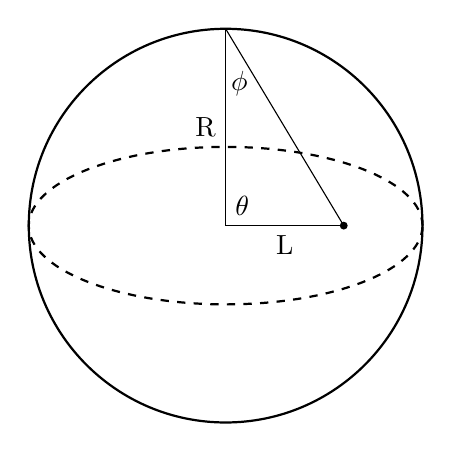
\begin{tikzpicture}[scale=0.5]
        \draw[thick] (0,0) circle(5);
        \draw[thick,dashed] (0,0) ellipse(5 and 2);

        \fill (3,0) circle[radius=0.1];

        \draw (0,0) -- node[below]{L} ++(3,0);
        \draw (3,0) -- (0,5);
        \draw (0,5) -- node[left]{R} (0,0);
        \node[above right] at (0,0) {$\theta$};
        \node[] at (0.35,3.6) {$\phi$};
    \end{tikzpicture}
    \caption{Sphere Integral}
    \label{sphere_integral}
\end{figure}

\begin{equation}
    f(t) = \frac{1}{\tau} e^{-\frac{t}{\tau}} \int_{\varphi} \int_{x = \cos{\theta}} e^{\frac{\sqrt{L^2-2 L R x+R^2}}{c
    \tau }} \frac{R^2 (R-L x)}{4\pi
    \left(L^2-2 L R x+R^2\right)^{3/2}} \\[2ex]
\end{equation}

The $\cos{\theta}$ integral requires care, because we can only integrate over
those parts of the sphere where it is possible for light to have made it, i.e.
we can only integrate over $\theta$ which satisfy

\[
    (c t)^2 \geq L^2-2 L R \cos{\theta} +R^2
\]

\newpage
The result is a piecewise function

\begin{equation}
    f(t) = \frac{1}{\tau} e^{-\frac{t}{\tau}}\left\{
    \begin{array}{l c}
        0 & \quad t < t_m \\[2ex]

        \frac{t_c \left(t \tau  e^{\frac{t_m}{\tau }}-t_m \left(t
        \text{Ei}\left(\frac{t_m}{\tau }\right)-t
        \text{Ei}\left(\frac{t}{\tau}\right)+\tau  e^{t/\tau }\right)\right)+t \tau ^2
        \left(e^{t/\tau }-e^{\frac{t_m}{\tau }}\right)}{2 t \tau\left(t_c-t_m\right)}
        & \quad
        t_m < t < t_c \\[2ex]

        \frac{t_c \left(t_m \left(\text{Ei}\left(\frac{t_c}{\tau
        }\right)-\text{Ei}\left(\frac{t_m}{\tau }\right)\right)+\tau e^{\frac{t_m}{\tau
        }}\right)+\tau  \left(e^{\frac{t_c}{\tau }} \left(\tau -t_m\right)-\tau
        e^{\frac{t_m}{\tau }}\right)}{2\tau  \left(t_c-t_m\right)}
        & \quad
        t > t_c
    \end{array} \right. \\[2ex]
    \label{f_t}
\end{equation}

where $\text{Ei}(x)$ is the
\href{http://en.wikipedia.org/wiki/Exponential_integral}{exponential integral function}, and $t_m$ and $t_c$ are defined as
\begin{align*}
    t_m &= \frac{R-L}{c} \\[2ex]
    t_c &= \frac{R+L}{c}
\end{align*}
and represent the time it would take a photon to travel the shortest and
longest distances to the sphere respectively. Note that although the expression
in Equation~\ref{f_t} looks complicated, it is only the terms involving $t$
that are really important. In particular, for $t > t_c$, $f(t)$ is nothing but
an exponential; all the terms right of the bracket are just normalizations. The
reason for this is that after light has had a chance to reach all parts of the
detector, everything arriving appears as an exponential with time constant
$\tau$ due to the memoryless-ness of the exponential distribution.

We can simplify Equation~\ref{f_t} considerably when the argument of the
exponential integral is large. In this case we can expand it asymptotically
around $\infty$. To second order in this expansion,

\begin{equation*}
    \text{Ei}(x) = e^x \left(\frac{1}{x^2}+\frac{1}{x}\right)
\end{equation*}

Expanding $\text{Ei}(x)$ to second order in $f(t)$, we get

\begin{equation}
    f(t) = \frac{1}{\tau} e^{-\frac{t}{\tau}}\left\{
    \begin{array}{l c}
        0 & \quad t < t_m \\[2ex]

        \frac{\tau  t_m e^{t/\tau } \left(t_c t_m+t^2\right)-t^2 \tau
        \left(t_c+t_m\right) e^{\frac{t_m}{\tau }}}{2 t^2 t_m\left(t_c-t_m\right)}
        & \quad
        t_m < t < t_c \\[2ex]

        \frac{\tau  \left(t_c+t_m\right) \left(t_m e^{\frac{t_c}{\tau }}-t_c
        e^{\frac{t_m}{\tau }}\right)}{2 t_c t_m\left(t_c-t_m\right)}
        & \quad
        t > t_c
    \end{array} \right. \\[2ex]
\end{equation}

To test the form of Equation~\ref{f_t}, I wrote a simple Monte Carlo.  I used
values close to those for SNO+ for the scintillation time and detector radius.
A plot of the hit time distribution for an event at a radius of 10m is shown in
Figure~\ref{hit_time_10} along with Equation~\ref{f_t}.

\begin{figure}[h!]
    \centering
    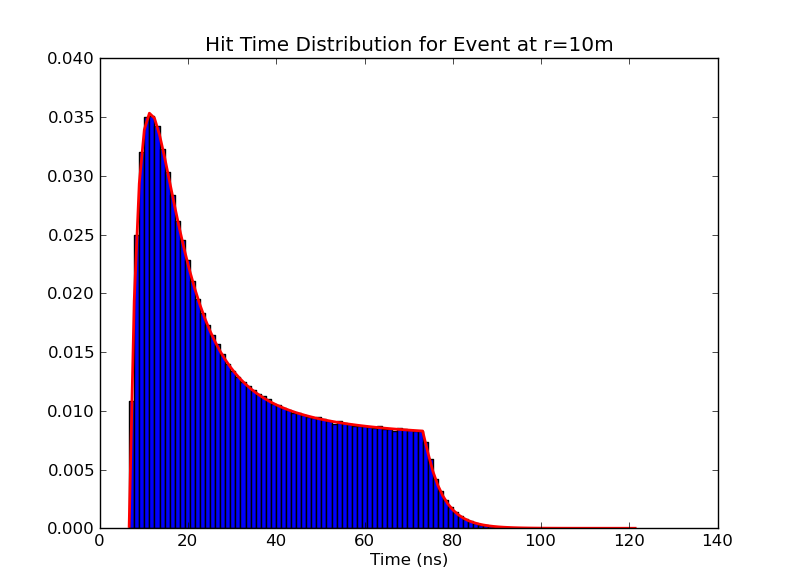
\includegraphics[width=0.75\linewidth]{hit_time_10.png}
    \caption{Time Distribution for Event at R=10m}
    \label{hit_time_10}
\end{figure}

\section{Fitting}
We can use Equation~\ref{f_t} to fit for the radius of an event from
\emph{nothing but the hit time distribution}. We construct a likelihood
function from Equation~\ref{f_t}

\[
    \like(L) = \prod_i f(t_i)
\]

A sample implementation is shown in Section~\ref{sample}. The resolution
as a function of the number of hits is shown in Figure~\ref{scint_res}
for events at a radius of 0, 1, and 6m. The first three lines use the above
equation, while the three lines labeled ``Full'' use a full likelihood fit in
three dimensions. It is interesting to note that the full likelihood resolution
does not depend on the radial distance of the event.  The reason for this is
that the hit distribution flattens out as the radius of the event increases,
and so the resolution decreases if you are only looking at the hit time
distribution. When fitting in three dimensions, the likelihood effectively
``sees'' the underlying exponential distribution, and therefore the resolution
increases.

\begin{figure}[h!]
    \centering
    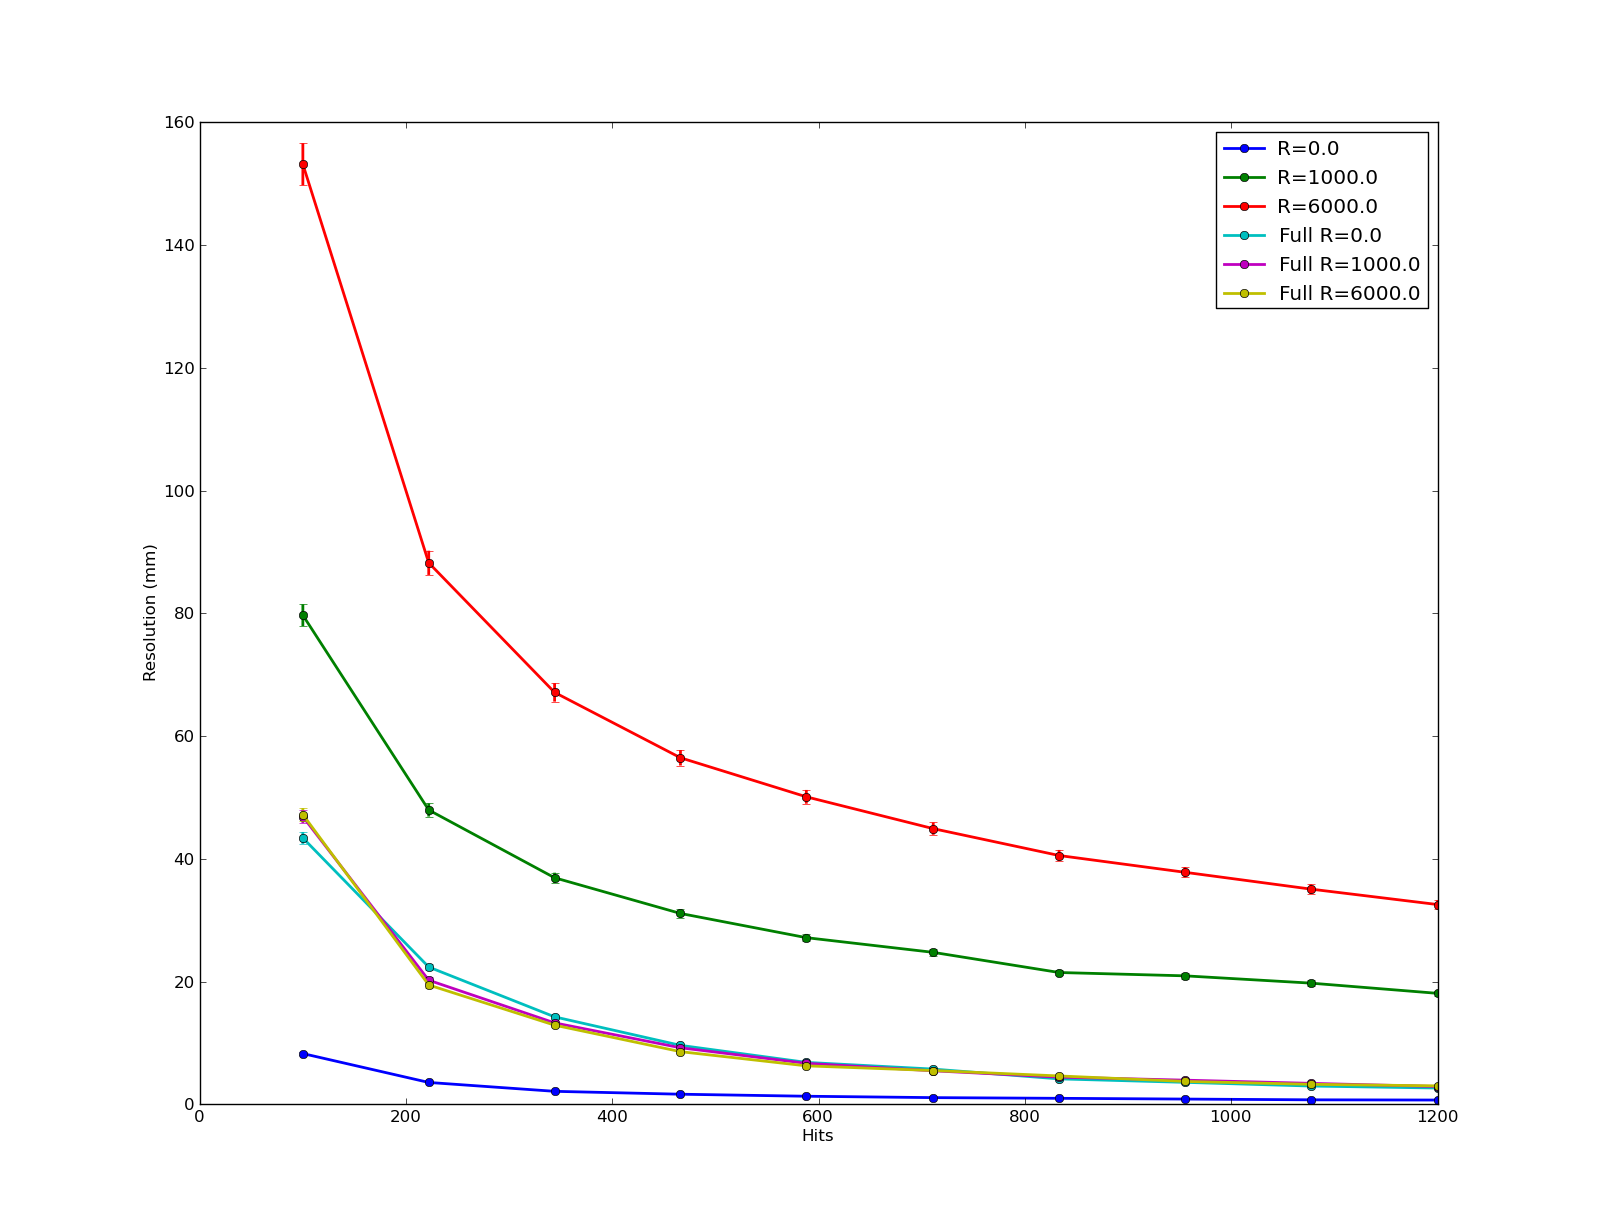
\includegraphics[width=1.0\linewidth]{../scint_res.png}
    \caption{Resolution as a function of Hits}
    \label{scint_res}
\end{figure}

\newpage
\section{Filter}
Given a set of hit times, we can calculate a KS test statistic for a
hypothesized (or fit) value of $L$, the radial distance of the event. A scatter
plot of the KS test statistic for 1,000 events as a function of the number of
hits for light coming from several different sources is shown in
Figure~\ref{ks_test}. The real events were generated with a true radial
position drawn randomly between 0 and 6m, the radial position was then fit, and
the KS test statistic evaluated at the fit radial distance. The photon bomb
events were generated near the edge of the detector at 10m, and the KS
statistic was computed at a radial distance of 6m, at the edge of the acrylic
vessel. The idea was to mimick a flashing PMT that had accidentally fit just
within the acrylic vessel. The random times were distributed uniformly over a
100ns interval, fit for a best radius, and the KS statistic was evaluated
there. The gaussian data was generated just like a real scintillation event,
but with normally distributed initial times.

\begin{figure}[h!]
    \centering
    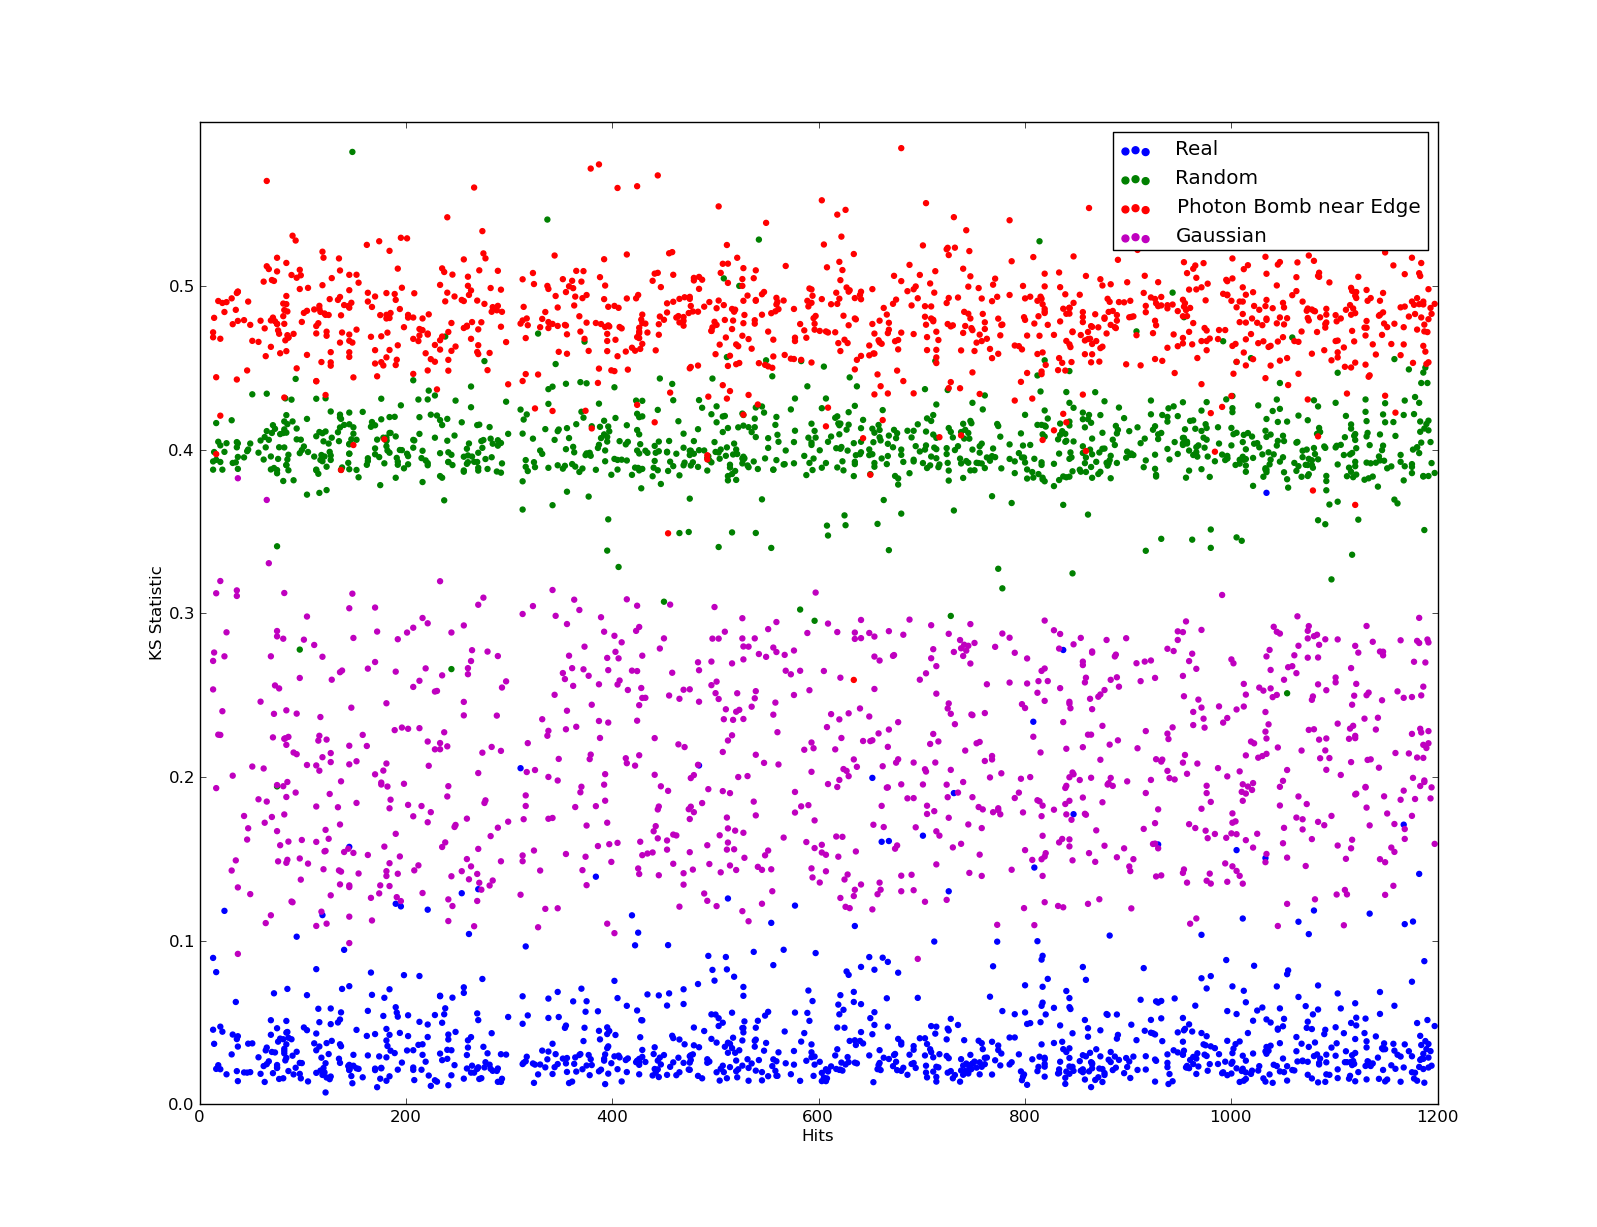
\includegraphics[width=1.0\linewidth]{../ks_test.png}
    \caption{KS Test}
    \label{ks_test}
\end{figure}

\clearpage
\section{Sample Implementation}
\label{sample}
\begin{multicols}{2}
    \inputminted[mathescape,linenos,numbersep=5pt,framesep=2mm,fontsize=\tiny]
    {python}{snotpos_minimal.py}
\end{multicols}

\end{document}
